% ----------------------------------------------------
% Appendix A4
% ----------------------------------------------------
\documentclass[class=report,11pt,crop=false]{standalone}
\input{../Style/ChapterStyle.tex}
\input{../FrontMatter/Glossary.tex}
\begin{document}
	% ----------------------------------------------------
	\chapter{Appendix A4}
	\subsection{Amplifier Test}
	The input into the amplifier was connected to the waveform generator on the oscilloscope. The input was set to 0V DC and the potentiometer was adjusted until the measured output on the oscilloscope was also 0. The output to the Arduino was then measured using a multimeter. This was repeated for different input values until the output saturated. This was also compared to the ideal output given by the following expression.
	\begin{center}
		$V_{out}=\frac{1}{2}\left(994V_{in} + 3.3\right)$ \\
	\end{center}
	
	The measurement for the output when the input was 1mV DC can be seen in Figure \ref{fig:S8} below. 
	\begin{figure}[h!]
		\centering
		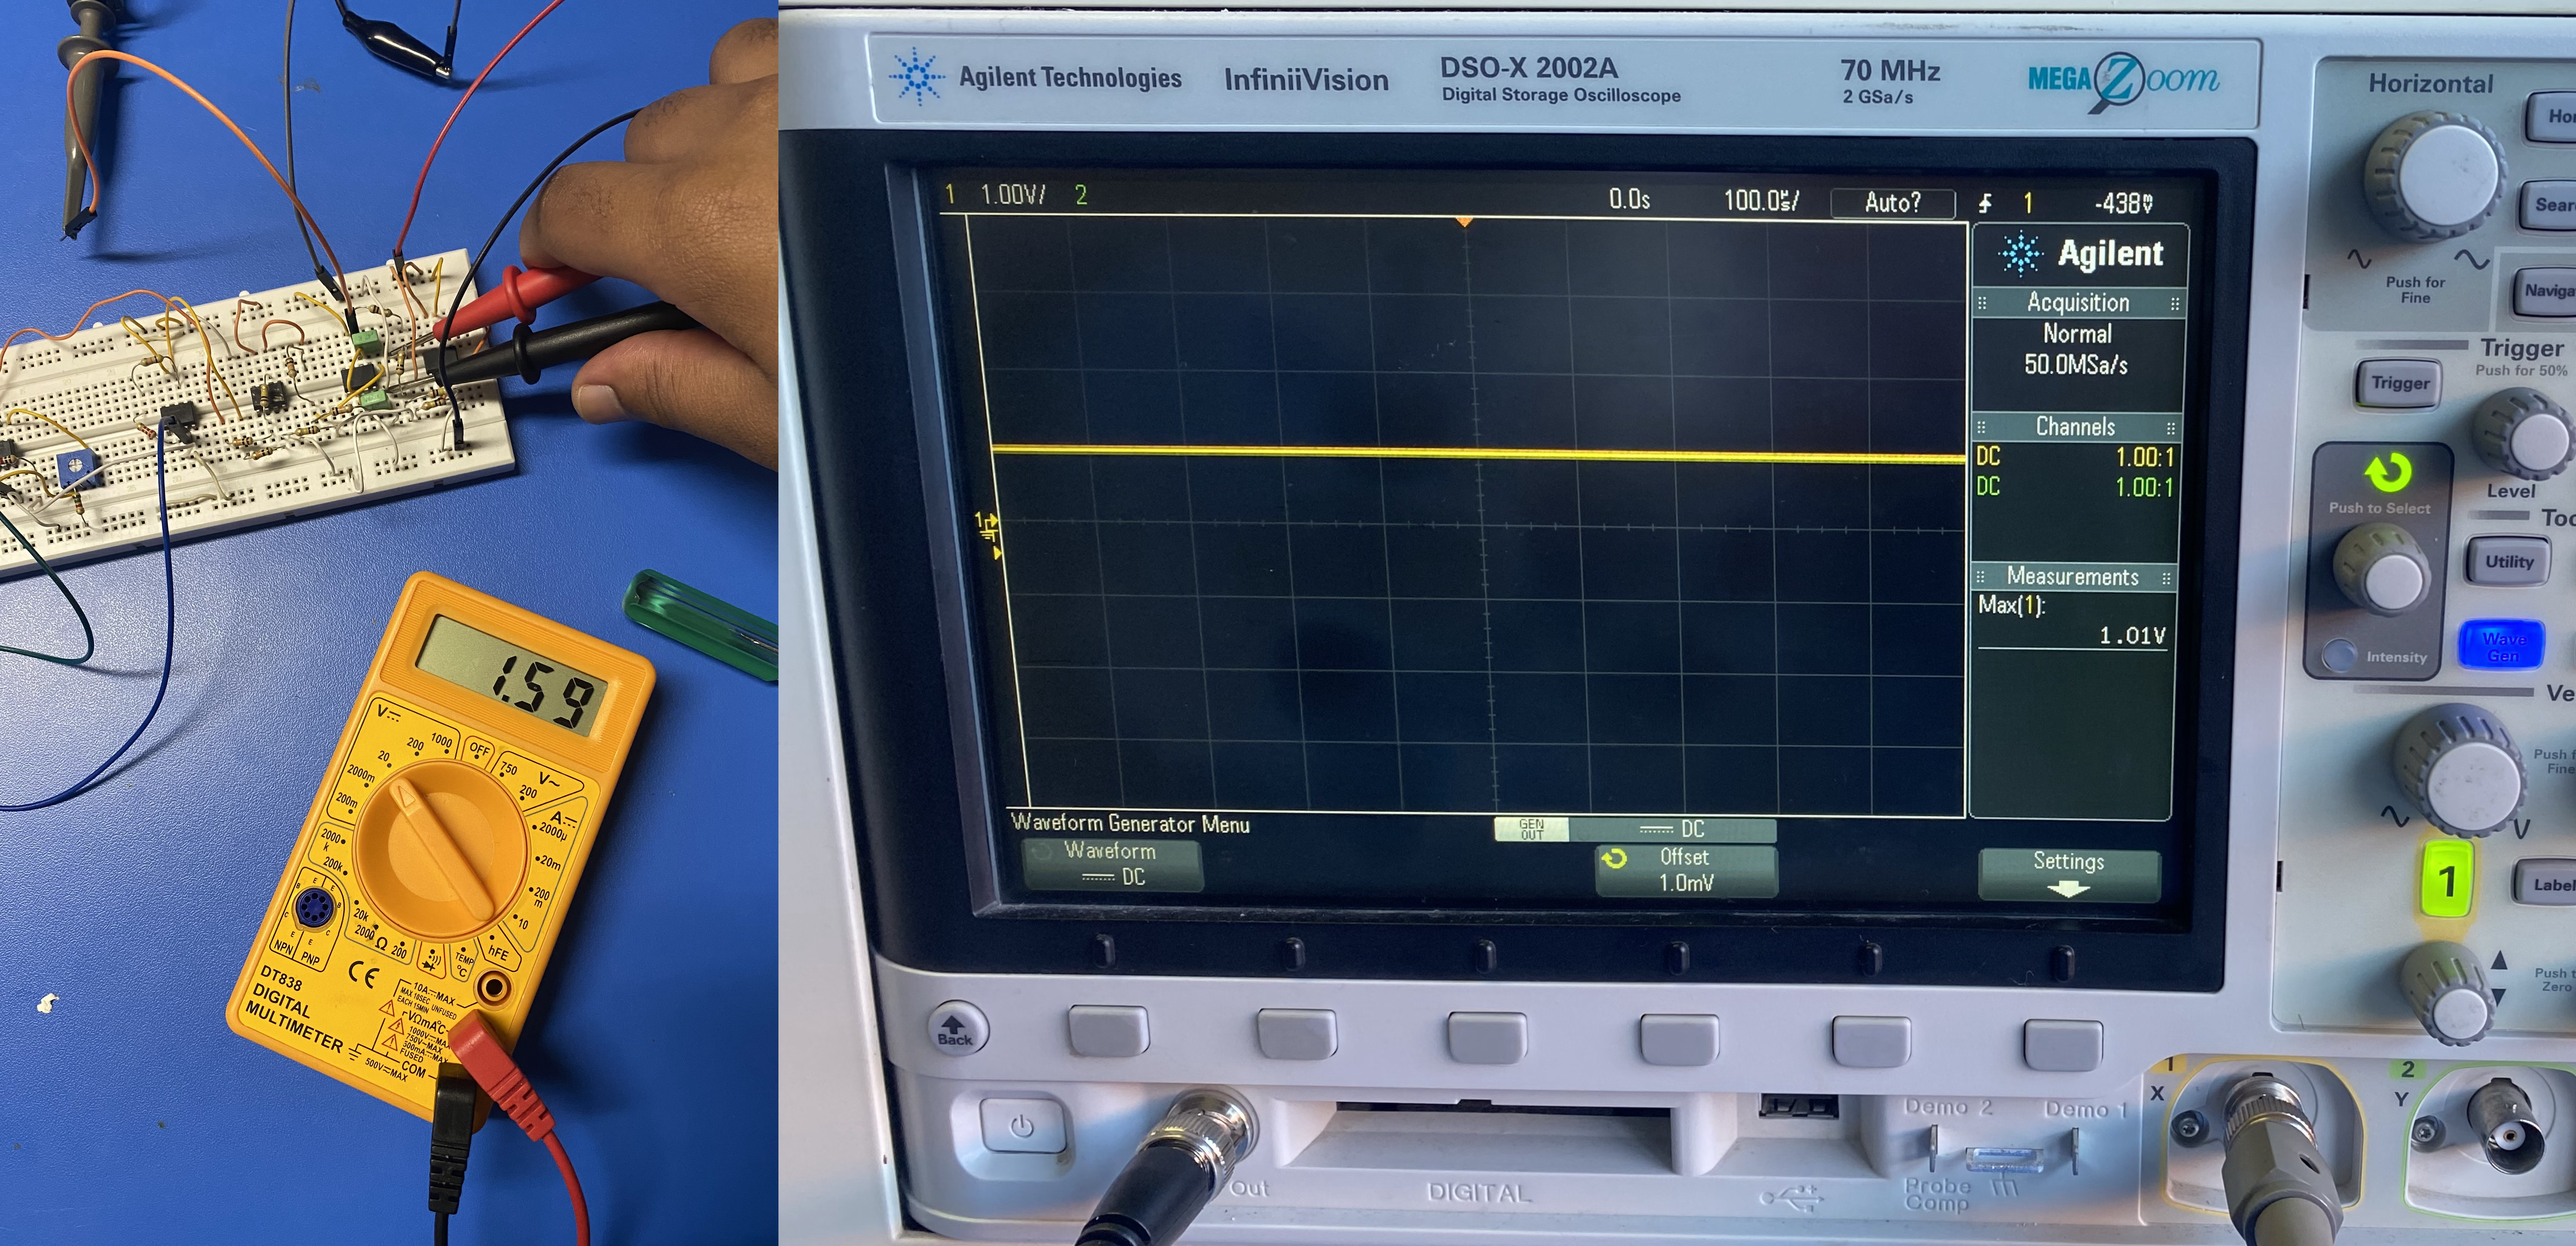
\includegraphics[width=0.8\linewidth]{Figures/ATP2.jpeg}
		\caption{Image of Amplifier test when input is 1mV}
		\label{fig:S8}
	\end{figure}
	
	The resulting plot of the output voltage against the input voltage from the oscilloscope is shown in Figure \ref{fig:S11} below.
	\begin{figure}[h!]
		\centering
		\includegraphics[width=0.4\linewidth]{Figures/Result1.png}
		\caption{Plot of Output voltage against input voltage from the oscilloscope}
		\label{fig:S11}
	\end{figure}
	% ----------------------------------------------------
	\ifstandalone
	\bibliography{../Bibliography/References.bib}
	\printnoidxglossary[type=\acronymtype,nonumberlist]
	\fi
\end{document}
% ----------------------------------------------------